\documentclass[a4paper,12pt,oneside,English]{article}
\usepackage[a4paper,top=1.5cm,bottom=1.5cm,left=1cm,right=1cm]{geometry}
\usepackage[utf8]{inputenc}
\usepackage[T1]{fontenc}
\usepackage{blindtext}
\usepackage{framed}
\usepackage[svgnames]{xcolor}
\usepackage{graphicx}
\definecolor{shadecolor}{gray}{0.9}
\usepackage{mathtools}
\usepackage{caption}
\usepackage{subcaption}
\usepackage{dsfont}
\usepackage{nccmath}
\usepackage{graphicx}
\usepackage{amsthm}
\usepackage{color} 
\usepackage[pdftex,backref,linktocpage,colorlinks]{hyperref}
\usepackage{xcolor}
\usepackage{empheq}
\usepackage{adjustbox}
\usepackage{graphicx}
\usepackage{amssymb}
\usepackage{amsmath}
\usepackage{siunitx}
\usepackage{framed}
\usepackage{graphicx}
\documentclass[xcolor=table]{beamer}
\usepackage[table,xcdraw]{xcolor}
\usepackage[authoryear]{natbib}
\hypersetup{
    colorlinks,
    linkcolor={red!50!black},
    citecolor={red!50!black},
    urlcolor={red!50!black}
}
\usepackage{titling}
\usepackage{fancyhdr}
\usepackage[shortlabels]{enumitem}
\usepackage{float}
\usepackage[nottoc, notlof]{tocbibind}
\usepackage{setspace}
\usepackage[T1]{fontenc}
\usepackage{amsfonts}
\usepackage{amsmath}
\usepackage{indentfirst}
\renewcommand{\baselinestretch}{1.5}
\setlength{\skip\footins}{5ex plus 4pt minus 2pt}
\usepackage{rotating}
\usepackage{tocloft}
\setlength{\cftaftertoctitleskip}{1cm}
\setlength{\cftafterloftitleskip}{1cm}
\usepackage{enumitem}
\usepackage{titletoc,tocloft}
\setlength{\cftsubsecindent}{0cm}
\usepackage{floatflt} 
 \usepackage[bf, small]{caption}
 \usepackage[justification=centering]{caption}
 \setcounter{secnumdepth}{0}
\title{Problem Set 1 - Econometrics}
\author{ Giacomo Lo Conte, Kun Wu, Francesca Eustacchi, Neeharika Kakunuri, Noor Ahmed Khoso }

\begin{document}
\maketitle
\section{ 1 Theory I: DAGs and Potential Outcomes}
\textbf{a) Consider the following threshold model with a binary treatment $D$, an additional (binary) covariate} $x$\textbf{, the outcome} $y$ \textbf{and an i.i.d error term with mean zero} $\epsilon_i$
\begin{equation}
    y_i = \alpha + \beta D_i + \gamma x_i + \rho \epsilon_i
\end{equation}
\begin{equation}
\label{eqn 2}
 x_i = \mathds{1}(\kappa + \delta D_i + \pi \epsilon_i > c) 
\end{equation}

\textbf{The second part of equation \ref{eqn 2} means that} $x_i = 1$ \textbf{if the sum on the right hand side is greater than a threshold c and $x_i = 0$ otherwise. Assuming that} $\delta = 0$\textbf{, show that the estimator of the average treatment effect (ATE), }$\Delta=E(y|D = 1 ,x = X) - E(y|D = 0 ,x = X)$ \textbf{equals}  $\beta$ + \textit{bias}\textbf{, characterise the bias (i.e. derive the exact formula)  and explain what the bias means.}\\

Consider the expected value of $y$ conditioned to $x=X$ and $D=0$ or $D=1$. 
\begin{equation}
\begin{split}
        y_{D=1}&=E[y|D=1, x=X]=E[\alpha+\beta+\gamma x + \rho \epsilon|D=1, x=X]\\
        y_{D=0}&=E[y|D=0, x=X]=E[\alpha+\gamma x + \rho \epsilon | D=0, x=X]\\
\end{split}
\end{equation}

\begin{equation}
\begin{split}
        y_{D=1}&=E[y|D=1, x=X]=\alpha+\beta+\gamma E[x|D=1, x=X] + \rho E[\epsilon|D=1, x=X]\\
        y_{D=0}&=E[y|D=0, x=X]=\alpha+\gamma E[x|D=0, x=X] + \rho E[\epsilon | D=0, x=X]\\
\end{split}
\end{equation}

Since $\delta=0$, $E[x|D]=E[\mathds{1}(\kappa+\pi\epsilon>c)|D]=E\Bigl[\mathds{1}\Bigl(\epsilon>\frac{c}{\pi}\Bigr)|D\Bigr]$ both when $D=1$ and $D=0$. The equation of $\Delta$ can be written as:
\begin{equation}
    \Delta=\alpha+\beta+\gamma E[x|D] + \rho E[\epsilon|D=1, x=X]-\alpha-\gamma E[x|D]-\rho E[\epsilon|D=0, x=X]
\end{equation}

Cancelling out the equal terms, it becomes:
\begin{equation}
    \Delta=\beta+\rho (E[\epsilon|D=0,x=X]-E[\epsilon|D=1,x=X])=\beta+\,bias
\end{equation}

If the error term is correlated with the treatment, then the term in parentheses is different from 0 and it will be a bias. This is a selection bias since the outcome across the two groups is influenced by unobservable variables correlated with the treatment captured by the error term. The sign of the bias is positive if these variables impact the outcome in the same direction the treatment affect them. Otherwise it will be negative.

\textbf{b) Now assume that }$\delta \neq 0$\textbf{. Write down a DAG that represents the model. Should the researcher account for }$x$ \textbf{to deconfound the treatment effect?}\\

\begin{figure}[h!]
    \centering
    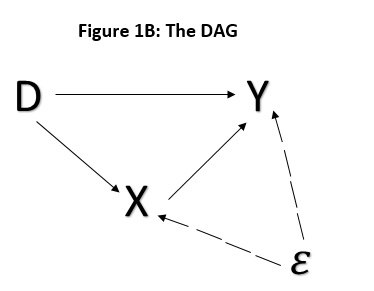
\includegraphics[width=0.5\textwidth]{Figure 1B.png}
    \caption{DAG of the theoretical model}
    \label{fig 1}
\end{figure}

The researcher should not account for $x$ to deconfound the treatment effect because $x$ is a mediator, and thus conditioning on it would lead to a selection bas. In this case, $x$ is not as good as randomly assigned because it is a function of D.

\textbf{c) Now assume that }$\delta \not= 0$ \textbf{and} $\gamma = 0$\textbf{. Using the potential outcomes framework, show that the bias} $E(y|D = 1,x = X) - E(y|D = 0,x = X) - \beta$ \textbf{can be re-written as a weighted average of} $E(\epsilon|D=1,x=X)-E(\epsilon|D=0,x=X)$ \textbf{across group switch }$x=1$ \textbf{and} $x=0$\textbf{. Provide a brief interpretation of the bias term.}\\

Compute $\Delta=E(y|D = 1,x = X) - E(y|D = 0,x = X)$, when $\gamma=0$.

\begin{equation}
\label{eq_parent}
\begin{split}
    \Delta &= E[\alpha + \beta + \rho\epsilon | D=1, x=X] - E[\alpha + \rho\epsilon | D=0, x=X]\\
    \Delta &= \beta + \rho(E[\epsilon|D=1, x=X]-E[\epsilon|D=0, x=X])
\end{split}
\end{equation}

Consider now the term in parentheses in equation \eqref{eq_parent}. Notice that $x$ can assume only two values 1 and 0, then we can rewrite $E[\epsilon|x=X]$ as $E[\epsilon|x=1\cup x=0]$. Since this represents the union of the two possible events ($x$ is either 0 or 1, but it can never be something different from this), we can split the condition based on the frequency they appear in the dataset with.
\begin{equation}
\begin{split}
    E[\epsilon|D=1, x=X]-E[\epsilon|D=0, x=X]&=E[\epsilon|D=1, x=1]\cfrac{E[x=1|X]}{E[x=X]}+E[\epsilon|D=1, x=0]\cfrac{E[x=0|X]}{E[x=X]}-\\&+E[\epsilon|D=0, x=1]\cfrac{E[x=1|X]}{E[x=X]}+E[\epsilon|D=0, x=0]\cfrac{E[x=0|X]}{E[x=X]}
\end{split}
\end{equation}

Since $E[x]=E[x=1|X]+E[x=0|X]$, we can write $p=\frac{E[x=1|X]}{E[x]}$ and $1-p=\frac{E[x=0|X]}{E[x]}$. The previous equation then can be rewritten as:
\begin{equation}
    \begin{split}
    E[\epsilon|D=1, x=X]-E[\epsilon|D=0, x=X]&=p\Biggl(E[\epsilon|D=1, x=1]-E[\epsilon|D=0, x=1]\Biggr)+\\&+(1-p)\Biggl(E[\epsilon|D=1, x=0]-E[\epsilon|D=0, x=0]\Biggr)
\end{split}
\end{equation}

Notice that $p$ is less or equal than 1 and greater or equal than 0. Moreover they sum to 1. Such a difference can be interpreted as a weighted mean of the difference $\Delta_E=E[\epsilon|D=1, x=X]-E[\epsilon|D=0, x=X]$ across $x=0$ and $x=1$ groups. Now consider $\Delta$ again. As we proved $\Delta=\beta+\rho\Delta_E\Rightarrow\rho\Delta_E=\Delta-\beta$. Considering that $\rho$ is a constant, we can write $\rho E[\epsilon]=E[\rho\epsilon]=E[e]$. Then it becomes:
\begin{equation}
\begin{split}
        E(y|D = 1,x = X) - E(y|D = 0,x = X)-\beta
=p&\Biggl(E[e|D=1, x=1]-E[e|D=0, x=1]\Biggr)+\\(1-p)&\Biggl(E[e|D=1, x=0]-E[e|D=0, x=0]\Biggr)
\end{split}
\end{equation}



\textbf{d) Suppose }$\beta > 0$\textbf{. Derive conditions under which the inclusion of $x$ would lead to the underestimation of} $\beta$\textbf{, i.e.} $E(\hat\beta) < \beta$.

Consider the OLS estimator $\hat\beta$:
\begin{equation}
\begin{split}
\hat\beta&=\cfrac{Cov(y,D)}{Var(D)}=\cfrac{Cov(\alpha+\beta D + \gamma x + \rho \epsilon,D)}{Var(D)}\\
\hat\beta&=\cfrac{Cov(\alpha,D)}{Var(D)}+\cfrac{Cov(\beta D,D)}{Var(D)}+\cfrac{Cov(\gamma x,D)}{Var(D)}+\cfrac{Cov(\rho\epsilon,D)}{Var(D)}\\
\hat\beta&=\beta+\gamma\cfrac{Cov(x,D)}{Var(D)}+\rho\cfrac{Cov(\epsilon,D)}{Var(D)}
\end{split}
\end{equation}

Consider now the expected value of $\hat\beta$:
\begin{equation}
E[\hat\beta]=E\Biggl[\beta+\gamma\cfrac{Cov(x,D)}{Var(D)}+\rho\cfrac{Cov(\epsilon,D)}{Var(D)}\Biggr]=\beta + \gamma E\Biggl[\cfrac{Cov(x,D)}{Var(D)}\Biggr]   
\end{equation}

For $E[\hat\beta]<\beta$, we must have $\gamma E\Biggl[\cfrac{Cov(x,D)}{Var(D)}\Biggr]<0$. Consider then this last term:
\begin{equation}
    E\Biggl[\cfrac{Cov(x,D)}{Var(D)}\Biggr]=E\Biggl[\cfrac{Cov[\mathds{1}(\kappa+\delta D+\pi \epsilon),D]}{Var(D)}\Biggr]
\end{equation}

The sign of this term is given by the sign of $\delta$. So the conditions for it to be true is that either $\gamma>0$ and $\delta<0$ or $\gamma<0$ and $\delta>0$.

\newpage
\section{2 Theory and Simulation}
\subsection{2.1 The Gender Pay Gap}
\begin{figure}[h!]
    \centering
    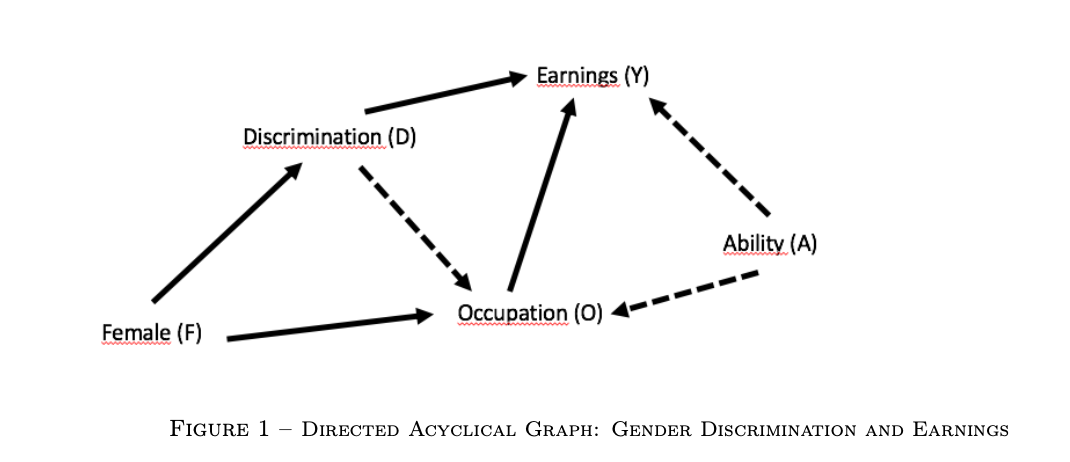
\includegraphics[width=0.5\textwidth]{Image 1.png}
    \caption{DAG of the theoretical model}
    \label{fig 2}
\end{figure}
\textbf{A researcher wants to estimate the effect of gender discrimination on earnings. To deconfound the causal effect, he/she develops the causal diagram shown in Figure \ref{fig 1}. All variables except A are observed in the data set. $F$ is a dummy variable that equals unity if a person is female. $0$ is a set of dummy variables for broad occupational categories. $D$ is a dummy variable indicating if a person is being discriminated or not. Assume that only women are discriminated against. The arrow from $D$ to $O$ is dashed because it is theoretically unclear whether we should expect an effect of discrimination on occupation.}\\
\textbf{a) Provide an intuitive explanation for each arrow in Figure \ref{fig 1}. Provide an explanation for the absence of an arrow between $F$ and $Y$ . In your view, should there be additional arrows and/or variables in the diagram? If so, which ones?}\\

\textbf{(a.1) Arrows Explanation}\\
\textbf{1. Female on Occupation (F-O)}\\
When O varies as F differs, it represents the changes in likelihood of having different choice range for occupation conditioning on gender. When a negative association presents, it implies that F=1 leads to decline in the likelihood of observing O=1, in which female is selected out in employment participation by gender disparities for given occupations. Instead of tangible economic reasons, preference over gender-specific occupations are introduced commonly by social norm or cultural belief. Outflow and inflow of self-selection presents when the gender-specific advantage is subjectively perceived for given occupations. Only a few extreme cases exist such as military service where being male has dominant conscription advantages against females. 

\textbf{2. Occupation on Earnings (O-Y)}\\
The potential variations for earnings given by occupation dummy provides a representation of the fact that different job categories get different earnings. When O is positively associated with Y, higher earnings are expected for a higher range of occupations, which are categorised as in O=1. Wages vary across occupations given by non-pecuniary characteristics of different jobs, compensation for skill training cost, institutional factor which obstructs the market equalisation of wage, hierarchy introduced by restricted access to resource and opportunities to limited circle of eligibility, valuation of personal natural ability and cognitive skills, and etc. The present occupation dummy implies a binary categorisation of aforementioned elements regarding the determination of wages.

\textbf{3. Female on Discrimination (F-D)}\\
When F is positively associated with D, the likelihood of presence of discrimination is higher for female than male on the basis of gender. When only gender is considered regarding discrimination behaviour, it links to the belief about a particular conceptualised masculinity and femininity. Acceptance and expectation derive from such social or cultural customs and norms and contribute to the gender stereotype, which lead to presence of gender superiority to another, primarily against female. The impact and severity of discrimination vary across societies, social groups, social roles, as well as vary at equality movement progress. 

\textbf{4. Discrimination on Earnings (D-E)}\\
Discrimination introduces the unjustified distinction in the variation of earnings conditioning on its presence. When the D is negatively correlated with E, to being discriminated against reduces the likelihood of having higher earnings. This implies an unequal treatment of indifferent productive individuals only because they belong to a specific group.

\textbf{5. Discrimination on Occupation (D-O)}\\
\textbf{6. Ability on Occupation (A-O)}\\
\textbf{7. Ability on Earnings (A-Y)}\\

\textbf{(a.2) Absence of an Arrow between F and Y}\\
Holding all the other factors fixed, when only the gender makes the earnings different, then this effect is captured by the presence of discrimination. When there is no discrimination, earnings are associated with the different payment for various occupations. Thus, the condition of having different earnings is fully explained by either the presence of discrimination or the difference in occupation, and the binary variable of gender alone cannot have no direct effect on earnings. If not sufficient, the unobservable ability variable captures all the rest of working performance that is undefined by the occupation type and discrimination behaviours.

\textbf{(a.2) Potential Additional Arrows}\\
The other potential additional variables/arrows that can be added would be education. Education as a variable has both direct and indirect impact on earnings. Note that in our example, we assume that ability is not correlated with education. We define in this particularly that ability can be intelligence and other characteristics of an individual, we can assume that abilities are characteristics that an individual possesses. On the other hand, education is acquired.

It is also worth mentioning that, discrimination also will have an impact on education which further impacts earnings. (DAG to be inserted) //Noor add if needed

Another possible extension would be to introduce is motherhood. It is very common and indeed a very much discussed possibility. Many instances of discrimination have been noted especially in studies that try to establish that motherhood often led to more discrimination towards women. Although many studies establish that  discrimination occurs to reduced ability - the general idea being females tend to be more distracted and have a lack of focus on their responsibilities. Thus, in
\textbf{b) Write out the paths from $D$ to $Y$ . Now assume that you observe ability and can control for it. Explain whether it makes sense (or not) to additionally control for the following: i) only $F$ ; ii) only $O$; iii) both.}\\
\textbf{c) Assume that $A$ is unobservable. Explain why controlling for $O$ can lead to collider bias.}\\
\textbf{d) Illustrate the collider problem in a simulation based on the above causal diagram. To do so, create a (simulated) dataset that represents all the arrows in Figure 1. It is sufficient to approximate O with one dummy variable. You will have to run several regressions; at the least, show the following regressions: i) $Y$ on $D$; ii) $Y$ on $D$ controlling for $O$; iii) $Y$ on $D$ controlling for $O$ and $A$. Run further regressions if needed and explain why the coefficients differ (or not). The task is here to show convincingly that controlling for variables on the causal path can lead to collider bias. This is what researchers would do in methodological papers, conference discussions or referee reports.}

The data set simulated data set contains 1000 observations. We have used the tool R for simulating this data set. We have generated dummy variables for \textit{"Female"}, \textit{"Occupation"} and \textit{"Discrimination"}. To simulate our model we picked parameters $a=0.5$, $b=2$, $c=3$, $d=-1.2$, $e=-2.1$, $f=0.25$, $g=23.5$, $h=5.8$, $i=-3.03$ and $k=12.8$. The simulated model is described by the following set of equations:
\begin{equation}
    \begin{split}
        &Discrimination=\mathds{1}(a+b^*Female+u_D>2.8)\\
        &Occupation=\mathds{1}(c+d^*Discrimination+e^*Female+f^*Ability+u_O>7)\\
        &Earnings=g+h^*Ability+i^*Discrimination+k^*Occupation+u_E
    \end{split}
\end{equation}

Units of measurement are taken in euros.

\begin{table}[!htbp] \centering 
  \caption{Regression summary for Earnings on Discrimination} 
  \label{reg table 1}
  \begin{threeparttable}
  \begin{tabular}{@{\extracolsep{5pt}}lc} 
\\[-1.8ex]\hline 
\hline \\[-1.8ex] 
 & \multicolumn{1}{c}{\textit{Dependent variable:}} \\ 
\cline{2-2} 
\\[-1.8ex] & Earnings \\ 
\hline \\[-1.8ex] 
 Discrimination & $-$5.893$^{***}$ \\ 
  & (1.606) \\ 
  & \\ 
 Constant & 142.849$^{***}$ \\ 
  & (1.073) \\ 
  & \\ 
\hline \\[-1.8ex] 
Observations & 1,000 \\ 
R$^{2}$ & 0.013 \\ 
Adjusted R$^{2}$ & 0.012 \\ 
Residual Std. Error & 25.246 (df = 998) \\ 
F Statistic & 13.465$^{***}$ (df = 1; 998) \\ 
\hline 
\hline \\[-1.8ex] 
\textit{Note:}  & \multicolumn{1}{r}{$^{*}$p$<$0.1; $^{**}$p$<$0.05; $^{***}$p$<$0.01} \\ 
\end{tabular}
\hfill\parbox[t]{0.5\textwidth}{This table reports estimation results from an OLS Model of \textit{Earnings} on \textit{Discrimination}. Standard error reported in parentheses in column.}
\end{threeparttable}
\end{table} 
\\
In table \ref{reg table 1} , we see the summary of the regression for earnings upon discrimination. We see that the estimate of discrimination is significant at 1 percent. The estimate is $-5.893$ indicating that in the presence of discrimination, earning fall by 5.893 euros. However, when we compare the parameter \textit{i} which is associated with Discrimination , we that the decrease in wages is lesser than -3.03. 
\begin{table}[!htbp] \centering 
  \caption{Regression Summary for Earnings, Discrimination controlling for Occupation} 
  \label{reg table 2}
  \begin{threeparttable}
  \begin{tabular}{@{\extracolsep{5pt}}lc} 
\\[-1.8ex]\hline 
\hline \\[-1.8ex] 
 & \multicolumn{1}{c}{\textit{Dependent variable:}} \\ 
\cline{2-2} 
\\[-1.8ex] & Earnings \\ 
\hline \\[-1.8ex] 
 Discrimination & $-$3.231$^{**}$ \\ 
  & (1.426) \\ 
  & \\ 
 Occupation & 26.543$^{***}$ \\ 
  & (1.574) \\ 
  & \\ 
 Constant & 122.630$^{***}$ \\ 
  & (1.527) \\ 
  & \\ 
\hline \\[-1.8ex] 
Observations & 1,000 \\ 
R$^{2}$ & 0.232 \\ 
Adjusted R$^{2}$ & 0.231 \\ 
Residual Std. Error & 22.279 (df = 997) \\ 
F Statistic & 150.887$^{***}$ (df = 2; 997) \\ 
\hline 
\hline \\[-1.8ex] 
\textit{Note:}  & \multicolumn{1}{r}{$^{*}$p$<$0.1; $^{**}$p$<$0.05; $^{***}$p$<$0.01} \\ 
\end{tabular}
\hfill\parbox[t]{0.5\textwidth}{This table reports estimation results from an OLS Model of \textit{Earnings} on \textit{Discrimination} and \textit{Occupation}. Standard error reported in parentheses in column.}
\end{threeparttable}
\end{table} 

In table \ref{reg table 2} we see the summary of regression of the effect of discrimination on earnings while controlling for occupation. The estimates are significant at 1 percent. And interestingly we see that earnings reduce by 3.231 which is significant with the set  parameter \textit{i} which is 3.03 units. With an increase in the occupational categories, we witness that earnings increase by 25.543 euros. Additionally, the explanatory power has now increased from 0.013 from regression 1 in table \ref{reg table 1} to 0.231. 

\begin{table}[!htbp] \centering 
  \caption{Regression Summary for Earnings , Discrimination controlling for occupation and ability} 
  \label{reg table 3}
  \begin{threeparttable}
  \begin{tabular}{@{\extracolsep{5pt}}lc} 
\\[-1.8ex]\hline 
\hline \\[-1.8ex] 
 & \multicolumn{1}{c}{\textit{Dependent variable:}} \\ 
\cline{2-2} 
\\[-1.8ex] & Earnings \\ 
\hline \\[-1.8ex] 
 Discrimination & $-$3.189$^{***}$ \\ 
  & (0.246) \\ 
  & \\ 
 Occupation & 12.771$^{***}$ \\ 
  & (0.282) \\ 
  & \\ 
 Ability & 5.799$^{***}$ \\ 
  & (0.032) \\ 
  & \\ 
 Constant & 39.634$^{***}$ \\ 
  & (0.531) \\ 
  & \\ 
\hline \\[-1.8ex] 
Observations & 1,000 \\ 
R$^{2}$ & 0.977 \\ 
Adjusted R$^{2}$ & 0.977 \\ 
Residual Std. Error & 3.845 (df = 996) \\ 
F Statistic & 14,200.460$^{***}$ (df = 3; 996) \\ 
\hline 
\hline \\[-1.8ex] 
\textit{Note:}  & \multicolumn{1}{r}{$^{*}$p$<$0.1; $^{**}$p$<$0.05; $^{***}$p$<$0.01} \\ 
\end{tabular}
\hfill\parbox[t]{0.5\textwidth}{This table reports estimation results from an OLS Model of \textit{Earnings} on \textit{Discrimination}, \textit{Occupation} and \textit{Ability}. Standard error reported in parentheses in column.}
\end{threeparttable}
\end{table}
In table \ref{reg table 3} we observe the summary of the regression earnings explained by discrimination while controlling for ability and occupation. The regression estimates are significant at 1 percent. Additionally, the models, explanatory power as explained by $R^2$ to 0.977. We also see that the coefficient of discrimination is -3.189 which is significant when compared to the parameter we have set.

Moreover, we see that the coefficient is more significant when compared to the coefficient we have obtained in regression 2, in table \ref{reg table 2}. Therefore, using the control for ability and occupation has improved our model, because, ability is a confounder in our model.

\begin{table}[!htbp] \centering 
  \caption{Regression Summary for Earnings and Discrimination while controlling for Ability and Occupation} 
  \label{reg table 4} 
\begin{tabular}{@{\extracolsep{5pt}}lc} 
\\[-1.8ex]\hline 
\hline \\[-1.8ex] 
 & \multicolumn{1}{c}{\textit{Dependent variable:}} \\ 
\cline{2-2} 
\\[-1.8ex] & Earnings \\ 
\hline \\[-1.8ex] 
 Discrimination & $-$3.189$^{***}$ \\ 
  & (0.246) \\ 
  & \\ 
 Occupation & 12.771$^{***}$ \\ 
  & (0.282) \\ 
  & \\ 
 Ability & 5.799$^{***}$ \\ 
  & (0.032) \\ 
  & \\ 
 Constant & 39.634$^{***}$ \\ 
  & (0.531) \\ 
  & \\ 
\hline \\[-1.8ex] 
Observations & 1,000 \\ 
R$^{2}$ & 0.977 \\ 
Adjusted R$^{2}$ & 0.977 \\ 
Residual Std. Error & 3.845 (df = 996) \\ 
F Statistic & 14,200.460$^{***}$ (df = 3; 996) \\ 
\hline 
\hline \\[-1.8ex] 
\textit{Note:}  & \multicolumn{1}{r}{$^{*}$p$<$0.1; $^{**}$p$<$0.05; $^{***}$p$<$0.01}
\end{tabular} 
\end{table}

\newpage
Furthermore, we have run additional regressions to estimate a casual relationships.
\begin{table}[!htbp] \centering 
  \caption{Regression Summary for Earnings , Discrimination and Ability} 
  \label{reg table 5} 
  \begin{threeparttable}
  \begin{tabular}{@{\extracolsep{5pt}}lc} 
\\[-1.8ex]\hline 
\hline \\[-1.8ex] 
 & \multicolumn{1}{c}{\textit{Dependent variable:}} \\ 
\cline{2-2} 
\\[-1.8ex] & Earnings \\ 
\hline \\[-1.8ex] 
 Discrimination & $-$4.373$^{***}$ \\ 
  & (0.428) \\ 
  & \\ 
 Ability & 6.193$^{***}$ \\ 
  & (0.054) \\ 
  & \\ 
 Constant & 43.002$^{***}$ \\ 
  & (0.918) \\ 
  & \\ 
\hline \\[-1.8ex] 
Observations & 1,000 \\ 
R$^{2}$ & 0.930 \\ 
Adjusted R$^{2}$ & 0.930 \\ 
Residual Std. Error & 6.720 (df = 997) \\ 
F Statistic & 6,639.879$^{***}$ (df = 2; 997) \\ 
\hline 
\hline \\[-1.8ex] 
\textit{Note:}  & \multicolumn{1}{r}{$^{*}$p$<$0.1; $^{**}$p$<$0.05; $^{***}$p$<$0.01} \\ 
\end{tabular}
\hfill\parbox[t]{0.5\textwidth}{This table reports estimation results from an OLS Model of \textit{Earnings} on \textit{Discrimination} and \textit{Ability}. Standard error reported in parentheses in column.}
\end{threeparttable}
\end{table}
In table \ref{reg table 5}

\begin{table}[!htbp] \centering 
  \caption{Regression Summary for Earnings, Occupation while controlling for Ability} 
  \label{reg table 6}
  \begin{threeparttable}
  \begin{tabular}{@{\extracolsep{5pt}}lc} 
\\[-1.8ex]\hline 
\hline \\[-1.8ex] 
 & \multicolumn{1}{c}{\textit{Dependent variable:}} \\ 
\cline{2-2} 
\\[-1.8ex] & Earnings \\ 
\hline \\[-1.8ex] 
 Occupation & 13.159$^{***}$ \\ 
  & (0.303) \\ 
  & \\ 
 Ability & 5.799$^{***}$ \\ 
  & (0.035) \\ 
  & \\ 
 Constant & 37.927$^{***}$ \\ 
  & (0.555) \\ 
  & \\ 
\hline \\[-1.8ex] 
Observations & 1,000 \\ 
R$^{2}$ & 0.973 \\ 
Adjusted R$^{2}$ & 0.973 \\ 
Residual Std. Error & 4.155 (df = 997) \\ 
F Statistic & 18,175.270$^{***}$ (df = 2; 997) \\ 
\hline 
\hline \\[-1.8ex] 
\textit{Note:}  & \multicolumn{1}{r}{$^{*}$p$<$0.1; $^{**}$p$<$0.05; $^{***}$p$<$0.01} \\ 
\end{tabular}
\hfill\parbox[t]{0.5\textwidth}{This table reports estimation results from an OLS Model of \textit{Earnings} on \textit{Occupation} and \textit{Ability}. Standard error reported in parentheses in column.}
\end{threeparttable}
\end{table} 
\newpage

\subsection{2.2  Application: Miscarriages and the Outcomes of Subsequent Children}
\textbf{In a new paper, the authors study the effect of a mother having a miscarriage on the outcomes of sub-sequent children. Prior research has shown that miscarriages, while common, can have traumatic effects on women and, by extension, on families. It is thus plausible that a miscarriage affects the outcomes of children that were subsequently conceived and born, for example through changes in parenting styles.
The authors undertake several steps towards establishing causality. They refer to a large number of studies showing that the likelihood of having miscarriages appear to be unrelated to mother or family characteristics, and provide balancing tests in support of this assumption. A second challenge is to find a suitable control group. They restrict the sample to families with two children; the treatment group had a miscarriage in between the births of both children, the control group had no miscarriage.}\\
\textbf{a) While this identification strategy appears plausible at first, the choice of control group may induce a bad control problem (i.e. the choice is equivalent to conditioning on a mediator). Construct a DAG to explain where the bad control problem could lie and why this might bias the estimates (Hint: it has to do with the decision to have another child after a miscarriage). Discuss under what conditions the assumption that having a miscarriage is random is sufficient for establishing causality.}\\

\begin{figure}[h!]
    \centering
    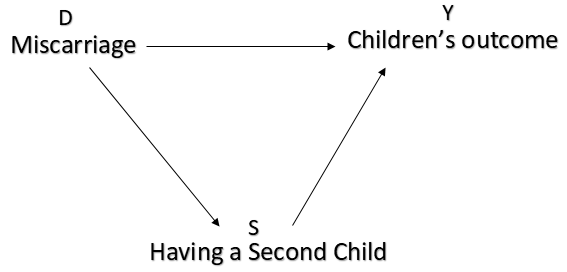
\includegraphics[width=0.5\textwidth]{Figure 2_2A1.png}
    \caption{DAG of the theoretical model}
    \label{fig 3}
\end{figure}
In this case, (S), which indicates the choice of having a second child is not as good as randomly assigned. In fact, S is a function of miscarriage. If we condition on S we could have an upward or downward bias, and both are plausible. In case of downward bias, we expect a direct effect of miscarriage on the decision to have a second child as negative. In this case, women who have had a miscarriage are less likely to have a second child, because they could have a traumatic shock related to the miscarriage that discourage them to tempt another pregnancy. Lower S would lead lower Y, but the effect would be reduced by the bias. 

In case of upward bias, we expect a direct effect of miscarriage on the decision to have a second child as positive. In this case, women who have had a miscarriage are more likely to have a second child, which could be explained by the fact that they are more mentally prepared because the consequence of the trauma of a miscarriage has already been addressed. Lower S would lead to lower Y, but the effect would be augmented by the bias.

The assumption of having miscarriage as random is sufficient for establishing causality if having a second child (S) is independent from having had miscarriage (D).

\textbf{b) Using potential outcomes notation, derive the bias in the estimation of the ATE that results from the bad control problem found in a). Explain in what direction the bias could likely go.}\\

In general, when we use the potential outcome notation, we define the casual effect of a treatment as the difference between the expected values of the outcome across the treatment and the control group:
\begin{equation}
    \Delta=E[Y|D=1]-E[Y|D=0]
\end{equation}

In the specific case, the author is controlling the treatment effects only for families with two children (S=1) and for those families who suffered a miscarriage between the two pregnancies. Suppose that the outcome is defined according the following Data Generating Process:
\begin{equation}
    Y=\alpha+\beta D + \gamma S + X'\delta + u
\end{equation}

The underlying assumption of the authors is that there is no selection bias in the estimation of the Average Treatment Effect, i.e.:
\begin{equation}
\begin{split}
    ATE=E[Y|D=1, S=1]-E[Y|D=0, S=1]&=\alpha + \beta +\gamma E[S|D=1] + E[X'|D=1]\delta\\&- \alpha -  \gamma E[S|D=0] - E[X'|D=0]\delta=\beta
\end{split}
\end{equation}

Even assuming that $E[X'|D=1]=E[X'|D=0]$, it is hard to justify that the number of children a couple decide to have is not affected by the treatment itself. Specifically, couples that suffered a miscarriage might be scared of having a new pregnancy. Moreover, a miscarriage might be caused by problems that are likely to affect future pregnancies too. For these reasons, we think that the effect of a miscarriage on the number of the child is negative, i.e. $E[S|D=1]<E[S|D=0]$, and the casual effect is:
\begin{equation}
    ATE=\beta+\gamma(E[S|D=1]-E[S|D=0])
\end{equation}

The sign of the bias then will be positive if $\gamma<0$ and negative otherwise. It is difficult to evaluate what is the impact of the number of child on parenting style-associated outcomes. On one hand parents can be more "expert" and can transfer their experience accumulated with the first children on the subsequent ones. On the other, parents may have less time to take care of more children.

\textbf{c) Propose tests that could potentially show that the bias is quantitatively unimportant (after all, no identification strategy is perfect; so showing that a bias does not matter is often what is needed). Please be brief here.}

The likelihood of having a second child it is possible to vary with the treatment. If the average number of children across the two groups in our data set is similar we can state that the bias is negligible. Moreover, if the latter difference is significant, we can still compare the average frequency of two-children families across the two groups conditioned to families with only two children. 

\end{document}
